\documentclass[landscape,final,columns=3]{baposter}
\usepackage{geometry}
\geometry{left=0.8in,right=0.8in,top=0.8in,bottom=0.8in}
\usepackage{times}
\usepackage{calc}
\usepackage{graphicx}
\usepackage{amsmath}
\usepackage{amssymb}
\usepackage{relsize}
\usepackage{multirow}
\usepackage{bm}
\usepackage{color}

\usepackage{amsmath}
\usepackage{amsfonts}
\usepackage{amsthm}
\usepackage{enumitem}
\usepackage{dsfont}
\usepackage[margin=1in]{geometry}
\usepackage{amssymb}
\usepackage{pifont}
\usepackage{mathtools}

\newtheorem{thm}{Theorem}
\newtheorem{lem}{Lemma}
\newtheorem{prop}{Proposition}
\newtheorem{conj}{Conjecture}
\newtheorem{cor}{Corollary}

\theoremstyle{definition}
\newtheorem{claim}{Claim}
\newtheorem{fact}{Fact}
\newtheorem{defn}{Definition}
\newtheorem*{remark}{Remark}

\newcommand{\N}{\ensuremath{\mathbb{N}}}
\newcommand{\Z}{\ensuremath{\mathbb{Z}}}
\newcommand{\Q}{\ensuremath{\mathbb{Q}}}
\newcommand{\R}{\ensuremath{\mathbb{R}}}
\newcommand{\C}{\ensuremath{\mathbb{C}}}
\newcommand{\F}{\ensuremath{\mathbb{F}}}
\newcommand{\AP}{\ensuremath{\mathcal{A}_{2^{n}}}}
\newcommand{\BP}{\ensuremath{\mathcal{B}_{2^{n}}}}
\newcommand{\CP}{\ensuremath{\mathcal{C}_{2^{n}}}}
\newcommand{\DP}{\ensuremath{\mathcal{D}_{2^{n}}}}
\newcommand{\EP}{\ensuremath{\mathcal{E}_{2^{n}}}}
\newcommand{\FP}{\ensuremath{\mathcal{F}_{2^{n}}}}

\newcommand{\E}{\ensuremath{\mathbb{E}}}
\newcommand{\1}{\ensuremath{\mathds{1}}}

\DeclareMathOperator{\Gal}{Gal}
\DeclareMathOperator{\Jac}{Jac}
\DeclareMathOperator{\Var}{Var}
\DeclareMathOperator{\Cov}{Cov}
\DeclareMathOperator{\Div}{Div}

\usepackage{graphicx}
\usepackage{multicol}

\usepackage{pgfbaselayers}
\pgfdeclarelayer{background}
\pgfdeclarelayer{foreground}
\pgfsetlayers{background,main,foreground}

\usepackage{helvet}
\usepackage{palatino}
\pagestyle{empty}
\newcommand{\captionfont}{\footnotesize}

\usepackage{xcolor}
\pagecolor[RGB]{255,254, 230}

\selectcolormodel{cmyk}

\graphicspath{{images/}}
\setlength{\columnsep}{0.7em}
\setlength{\columnseprule}{0mm}
\newcommand{\compresslist}{%
\setlength{\itemsep}{1pt}%
\setlength{\parskip}{0pt}%
\setlength{\parsep}{0pt}%
}

\begin{document}

\typeout{Poster Starts}
%by changing the values inside the curly brackets you can get new colors
\definecolor{mit}{cmyk}{0,.667,.667,.4}
\definecolor{wil}{cmyk}{0.5,1,0,.6}
\definecolor{silver}{cmyk}{0,0,0,0.3}
\definecolor{yellow}{cmyk}{0,0,0.9,0.0}
\definecolor{reddishyellow}{cmyk}{0,0.22,1.0,0.0}
\definecolor{black}{cmyk}{0,0,0.0,1.0}
\definecolor{darkYellow}{cmyk}{0,0,1.0,0.5}
\definecolor{darkSilver}{cmyk}{0,0,0,0.1}
\definecolor{lightyellow}{cmyk}{0,0,0.3,0.0}
\definecolor{lighteryellow}{cmyk}{0,0,0.1,0.0}
\definecolor{lightestyellow}{cmyk}{0,0,0.05,0.0}
\begin{poster}{
  grid=no,
  columns=3,
   colspacing=1em,
  bgColorOne=lighteryellow, %background inside the boxes
  bgColorTwo=lightestyellow, %background color
  borderColor=reddishyellow,
  headerColorOne=yellow,
  headerColorTwo=reddishyellow,
  headerFontColor=black,
  boxColorOne=lightyellow,
  boxColorTwo=lighteryellow,
  % Format of textbox
  textborder=roundedleft,
  % Format of text header
  eyecatcher=no,
  headerborder=open,
  headerheight=0.08\textheight,
  headershape=roundedright,
  headershade=plain,
  headerfont=\Large\textsf, %Sans Serif
  boxshade=plain,
  background=plain,
  linewidth=2pt
  }
  {
  }
{\bf{\textcolor{mit}{This Shit is Bananas: ``B-A-N-A-N-A-S''}} %title
  % Authors
{\rm \\ \large  Louis Gaudet, Nicholas Wawrykow, and Theodore Weisman \ \ \
 \textbf{Mentors:} Daniel Corey, David Jensen, and Dhruv Ranganathan \\
 SUMRY 2014,\ Yale University
  }}

  % University logo: change the CMU.jpeg to whatever picture you want and then uncomment this section
%  {
%   \makebox[8em][r]{
%      \begin{minipage}{16em}
%        \hfill
%        \includegraphics[height=6.5em]{mitsealY.eps}
%            \end{minipage}
%            \hspace{-1.35in}
%        \begin{minipage}{16em}
%        \hfill
%        \includegraphics[height=5.8em]{wilsealY.eps}
%            \end{minipage}
%         \hspace{-1.35in}
%        \begin{minipage}{16em}
%        \hfill
%        \includegraphics[height=5.8em]{cookie.eps}
%            \end{minipage}
%    }
%  }

  \tikzstyle{light shaded}=[top color=baposterBGtwo!30!white,bottom color=baposterBGone!30!white,shading=axis,shading angle=30]
     \newlength{\leftimgwidth}
     \setlength{\leftimgwidth}{0.78em+8.0em}

%%%%%%%%%%%%%%%%%%%%%%%%%%%%%%%%%%%%%%%%%%%%%%%%%%%%%%%%%%%%%%%%%%%%%%%%%%%%%%
%%% Now define the boxes that make up the poster
%%%---------------------------------------------------------------------------
%%% Each box has a name and can be placed absolutely or relatively.
%%% The only inconvenience is that you can only specify a relative position
%%% towards an already declared box. So if you have a box attached to the
%%% bottom, one to the top and a third one which should be in between, you
%%% have to specify the top and bottom boxes before you specify the middle
%%% box.
%%%%%%%%%%%%%%%%%%%%%%%%%%%%%%%%%%%%%%%%%%%%%%%%%%%%%%%%%%%%%%%%%%%%%%%%%%%%%%
    %
    % A colored circle useful as a bullet with an adjustably strong filling
    \newcommand{\colouredcircle}[1]{%
      \tikz{\useasboundingbox (-0.2em,-0.32em) rectangle(0.2em,0.32em); \draw[draw=black,fill=baposterBGone!80!black!#1!white,line width=0.03em] (0,0) circle(0.18em);}}


 
 %%%%%%%%%%%%%%%%%%%%%%%%%%%%%%%%%%%%%%%%%%%%%%%%%%%%%%%%%%%%%%%%%%%%%%%%%%%%%%
  \headerbox{{\bf{Acknowledgements}}}{name=ack,column=0,span=2,above=bottom}{
%%%%%%%%%%%%%%%%%%%%%%%%%%%%%%%%%%%%%%%%%%%%%%%%%%%%%%%%%%%%%%%%%%%%%%%%%%%%%%
  \smaller
  This research was conducted as part of the 2014 SUMRY program at Yale University.
}%

%%%%%%%%%%%%%%%%%%%%%%%%%%%%%%%%%%%%%%%%%%%%%%%%%%%%%%%%%%%%%%%%%%%%%%%%%%%%%%
  \headerbox{{{\bf{The Jacobian group of a graph}}}}{name=defs,column=0,row=0,above=ack}{
  
{\textcolor{purple}{\large{\bf{Divisors on a graph}}}} \vspace{0.05in}\\
Let $G$ be a finite, connected multigraph with no loop edges. Let $V(G),E(G)$ be the vertex and edge sets of $G$.

\begin{itemize}
\item a \textbf{divisor} is an element of $\Div(G)=\bigoplus_{v\in V(G)}\Z(v)$, the free abelian group generated by $V(G)$
\end{itemize}
We think of divisors as ``configurations of chips'' on the vertices of $G$, with group structure given by pointwise addition:

\begin{center}
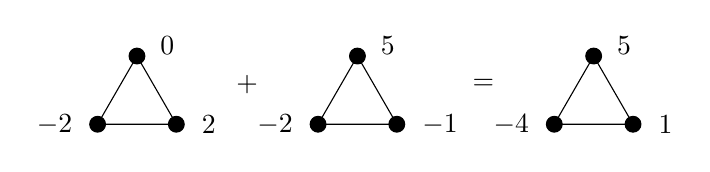
\begin{tikzpicture}

%first divisor
\draw (60:1) -- (0,0) -- (0:1) -- (60:1) ;

\draw [fill] (0,0) circle [radius=0.1cm] ;
\draw [fill] (60:1) circle [radius=0.1cm] ;
\draw [fill] (0:1) circle [radius=0.1cm] ;

%first divisor labels
\node [right] at (60:1.15) {$\;0$} ;
\node [left] at (-.1,0) {$-2\;$} ;
\node [right] at (0:1.2) {$2$} ;

%second divisor
\draw [shift={(2.8cm,0cm)}] (60:1) -- (0,0) -- (0:1) -- (60:1) ;

\draw [fill,shift={(2.8cm,0cm)}] (0,0) circle [radius=0.1cm] ;
\draw [fill,shift={(2.8cm,0cm)}] (60:1) circle [radius=0.1cm] ;
\draw [fill,shift={(2.8cm,0cm)}] (0:1) circle [radius=0.1cm] ;

%second divisor labels
\node [right,shift={(2.8cm,0cm)}] at (60:1.15) {$\;5$} ;
\node [left,shift={(2.8cm,0cm)}] at (-.1,0) {$-2\;$} ;
\node [right,shift={(2.8cm,0cm)}] at (0:1.2) {$-1$} ;

%resulting divisor
\draw [shift={(5.8cm,0cm)}] (60:1) -- (0,0) -- (0:1) -- (60:1) ;

\draw [fill,shift={(5.8cm,0cm)}] (0,0) circle [radius=0.1cm] ;
\draw [fill,shift={(5.8cm,0cm)}] (60:1) circle [radius=0.1cm] ;
\draw [fill,shift={(5.8cm,0cm)}] (0:1) circle [radius=0.1cm] ;

%resulting divisor labels
\node [right,shift={(5.8cm,0cm)}] at (60:1.15) {$\;5$} ;
\node [left,shift={(5.8cm,0cm)}] at (-.1,0) {$-4\;$} ;
\node [right,shift={(5.8cm,0cm)}] at (0:1.2) {$1$} ;

%plus and equals signs
\node [shift={(1.9cm,-.5cm)}] at (0,1) {$+$} ;
\node [shift={(4.9cm,-.5cm)}] at (0,1) {$=$} ;

\end{tikzpicture}
\end{center}

{\textcolor{purple}{\large{\bf{Chip-firing}}}} \vspace{0.05in}\\
You can ``fire'' a vertex on a divisor to get a new divisor:

\begin{center}
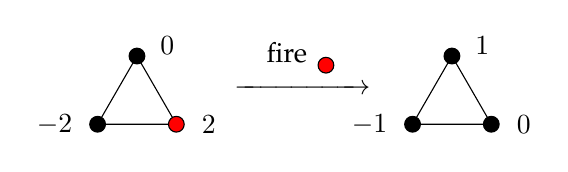
\begin{tikzpicture}

%first divisor
\draw (60:1) -- (0,0) -- (0:1) -- (60:1) ;

\draw [fill] (0,0) circle [radius=0.1cm] ;
\draw [fill] (60:1) circle [radius=0.1cm] ;
\draw [fill=red] (0:1) circle [radius=0.1cm] ;

%first divisor labels
\node [right] at (60:1.15) {$\;0$} ;
\node [left] at (-.1,0) {$-2\;$} ;
\node [right] at (0:1.2) {$2$} ;

%fire arrow
\node [shift={(2.6cm,-.5cm)}] at (0,1) {$\xrightarrow{\hspace{1.5cm}}$} ;
\node [above,shift={(2.6cm,-.5cm)}] at (0,1.15) {fire\;\;\;\;} ;
\draw [fill=red,shift={(2.9cm,1cm)}] (0,-.25) circle [radius=0.1cm] ;

%second divisor
\draw [shift={(4cm,0cm)}] (60:1) -- (0,0) -- (0:1) -- (60:1) ;

\draw [fill,shift={(4cm,0cm)}] (0,0) circle [radius=0.1cm] ;
\draw [fill,shift={(4cm,0cm)}] (60:1) circle [radius=0.1cm] ;
\draw [fill,shift={(4cm,0cm)}] (0:1) circle [radius=0.1cm] ;

%second divisor labels
\node [right,shift={(4cm,0cm)}] at (60:1.15) {$\;1$} ;
\node [left,shift={(4cm,0cm)}] at (-.1,0) {$-1\;$} ;
\node [right,shift={(4cm,0cm)}] at (0:1.2) {$0$} ;

\end{tikzpicture}
\end{center}

If you can get between two divisors $D$ and $D'$ via a sequence of chip-firing moves, then $D,D'$ are equivalent, $D\sim D'$.

\vspace{0.1in}

{\textcolor{purple}{\large{\bf{The Jacobian group}}}}
\begin{itemize}
\item $\deg(D)=$ the total number of chips in $D$
\item $\Div^0(G)=\{D\in\Div(G):\deg(D)=0\}$
\end{itemize}
Now we define the \textbf{Jacobian} group of the graph $G$:
\[
\Jac(G) = \Div^0(G)/\sim.
\]
For a finite graph $G$, $\Jac(G)$ is a finite abelian group.

\begin{prop}
$|\Jac(G)|=$ the number of spanning trees of $G$.
\end{prop}
This fact is a consequence of the Matrix Tree Theorem.

\vspace{0.1in}

 }

%%%%%%%%%%%%%%%%%%%%%%%%%%%%%%%%%%%%%%%%%%%%%%%%%%%%%%%%%%%%%%%%%%%%%%%%%%%%%%
 \headerbox{{\bf{Pairings on finite abelian groups}}}{name=pair,span=1,column=1,row=0}{
%%%%%%%%%%%%%%%%%%%%%%%%%%%%%%%%%%%%%%%%%%%%%%%%%%%%%%%%%%%%%%%%%%%%%%%%%%%%%%

Given a finite abelian group $\Gamma$, a \textbf{pairing} on $\Gamma$ is an inner-product like structure $\pair{\cdot}{\cdot}:\Gamma\times\Gamma \to \Q/\Z$ that is \emph{symmetric}, \emph{bilinear}, and \emph{non-degenerate}.

\vspace{0.1in}

{\textcolor{purple}{\large{\bf{Orthogonal sum}}}} \vspace{0.05in}\\
Given two groups $\Gamma_1,\Gamma_2$ with pairings $\pair{\cdot}{\cdot}_1,\pair{\cdot}{\cdot}_2$, the \textbf{orthogonal sum} is a natural pairing defined on $\Gamma_1\times\Gamma_2$ by
\[
\pair{(a_1,a_2)}{(b_1,b_2)}=\pair{a_1}{b_1}_1+\pair{a_2}{b_2}_2.
\]

}

%%%%%%%%%%%%%%%%%%%%%%%%%%%%%%%%%%%%%%%%%%%%%%%%%%%%%%%%%%%%%%%%%%%%%%%%%%%%%%
 \headerbox{{\bf{Pairings on $\Z/p^r\Z$}}}{name=prpair,span=1,column=2,row=0}{
%%%%%%%%%%%%%%%%%%%%%%%%%%%%%%%%%%%%%%%%%%%%%%%%%%%%%%%%%%%%%%%%%%%%%%%%%%%%%%

If $p$ is an odd prime, then, up to isomorphism, there are precisely two pairings on $\Z/p^r\Z$. Written additively, they are given by
\vspace{-0.15in}
\[
\pair{x}{y}=xy/p^r \quad \text{and} \quad \pair{x}{y}=axy/p^r,
\vspace{-0.05in}
\]
where $a$ is some quadratic nonresidue modulo $p^r$.

\vspace{0.1in}

{\textcolor{purple}{\large{\bf{Classification theorem}}}} \vspace{0.05in}\\
Given any pairing on any finite abelian group of \emph{odd} order, we can write it as the orthogonal sum of pairings on $\Z/p^r\Z$ terms.

}

%%%%%%%%%%%%%%%%%%%%%%%%%%%%%%%%%%%%%%%%%%%%%%%%%%%%%%%%%%%%%%%%%%%%%%%%%%%%%%
  \headerbox{{\bf{Pairings on $\Z/2^r\Z$}}}{name=2rpair,column=1, span=2, above=ack,below=pair,below=prpair}{
%%%%%%%%%%%%%%%%%%%%%%%%%%%%%%%%%%%%%%%%%%%%%%%%%%%%%%%%%%%%%%%%%%%%%%%%%%%%%%



}

\end{poster}%
%
\end{document}
